\documentclass[12pt]{article}
\usepackage{amsmath}
\usepackage{amsfonts}
\usepackage{amssymb}
\usepackage{physics}
\usepackage{graphicx}
\usepackage{hyperref}
\usepackage{subcaption}
\usepackage[
    backend=biber,natbib,
    % IMPORTANT: load a style suitable for your discipline
    style=nature
]{biblatex}
\addbibresource{c.bib}
\title{The Bethe-Salpeter Equation}
\author{Patryk Kozlowski}
\date{\today}
\begin{document}
\maketitle
\section{Mean field theory}
The central computational method in quantum chemistry is density functional theory (DFT). In their inaugural work, Hohenberg and Kohn proposed that the wave function for a system is uniquely determined by the electron density. Kohn and Sham then proposed a computational methodology that makes use of a self-consistent procedure, which is computationally cheap with a small scaling of $O(N^3)$, where $N$ is the number of electrons, and yet fairly accurate\autocite{bowler_calculations_2010}. It treats the quantum mechanical effects of the system by an exchange-correlation functional $V_{xc}$. This $V_{xc}$ is approximate and while you can get better approximations by moving up Jacob's ladder\autocite{milman_jacobs_2021}, it is difficult to systematically improve. Therefore, we turn to many-body perturbation theory (MBPT) which provides a framework to correct upon the properties predicted by DFT. In this work, we will consider the formalism of Green's functions within the framework of MBPT.
\section{Linear response theory}
Central to linear response theory is the random phase approximation, where one attempts to solve the matrix equation inspired by the operator introduced by \textcite{casida_progress_2012}
\begin{equation}
\hat{\mathcal{O}}^{\dagger}=\sum_{i, a} a^{\dagger} i X_{i a}+\sum_{i, a} i^{\dagger} a Y_{i a},
\label{eq: operator}
\end{equation}
where $i$ and $a$ are indices for occupied and virtual orbitals, respectively, and so by the definition of the second quantization operators, $X_{ia}$ and $Y_{ia}$ respond to excitations and de-excitations, respectively. We can then write a RPA matrix equation as \autocite{dreuw_single-reference_2005}
\begin{equation}
\begin{bmatrix}
\textbf{A} & \textbf{B} \\
-\textbf{B} & -\textbf{A}
\end{bmatrix}
\begin{bmatrix}
\textbf{X} \\
\textbf{Y}
\end{bmatrix}
=
\begin{bmatrix}
\textbf{X} \\
\textbf{Y}
\end{bmatrix}
\boldsymbol{\Omega }
,
\label{eq: RPA matrix equation}
\end{equation}
The matrices $\textbf{A}$ and $\textbf{B}$ correspond to the resonant and anti-resonant parts of the spectrum, respectively. From solving this eigenvalue equation, we can obtain the excitation and de-excitation energies (these are equal in magnitude but opposite in sign) of the system $\boldsymbol{\Omega}$ with the corresponding eigenvectors $\textbf{X}$ and $\textbf{Y}$, with elements corresponding to transitions given in equation \ref{eq:operator}. With the RPA, we are able to determine the weights of different excitations from occupied to virtual orbitals and vice versa, but this method does not describe the interactions between occupied and virtual states; this is needed to properly describe excitons, where a hole, described by an occupied orbital, is interacting with an electron, which resides in a virtual orbital\autocite{reining_10_nodate}. In order to describe excitons, one needs to turn to the Bethe-Salpeter equation, which resides within the Green's function formalism, which we will first introduce.

\section{Green's functions}
One can define the single-particle Green's function $G$ as
\begin{equation}
G\left(\mathbf{r}_1, t_1 ; \mathbf{r}_2, t_2\right)=-i\left\langle\Psi_0\left|T\left[\hat{\psi }\left(\mathbf{r}_1, t_1\right) \hat{\psi}^{\dagger}\left(\mathbf{r}_2, t_2\right)\right]\right| \Psi_0\right\rangle,
\label{eq:greens}
\end{equation}
where $ \hat{\psi}^{\dagger}(\hat{\psi})$ are the field operators for creating (destroying) a particle at spacetime coordinates $\mathbf{r}$ and $t$, $T$ is the time-ordering operator that ensures that the field operator at the earlier time is acting on the ket before the field operator at the later time, and $\Psi_0$ is the ground state wave function. The Green's function can be interpreted as measuring the probability that a particle created at $\mathbf{r}_2$ and $t_2$ will be destroyed at $\mathbf{r}_1$ and $t_1$. It is important to make the distinction between the noninteracting and interacting Green's functions of the system. The former means that the particles are not interacting as the name suggests and is usually defined by some mean field reference, like DFT, while the latter is really what we are after because we want to describe the scenario where the particles are interacting with each other, such as with not We can write down a Dyson equation\autocite{dyson_s_1949}, which relates the noninteracting Green's function to the interacting one symbolically as
\begin{equation}
G=G_0+G_0\Sigma G,
\label{eq:dyson}
\end{equation}
where we have introduced $\Sigma$, which is the self-energy operator. Isolating $\Sigma$, we get an illuminating definition of the self-energy as the difference between the inverses of the interacting and noninteracting Green's functions
\begin{equation}
\Sigma = G^{-1}-G_0^{-1}.
\end{equation}
The self-energy admits an intuitive physical picture. Consider the example of an electron shot into a gas of electrons, as shown in Figure \ref{fig:shot}.
\begin{figure}
\begin{subfigure}{.5\textwidth}
  \centering
  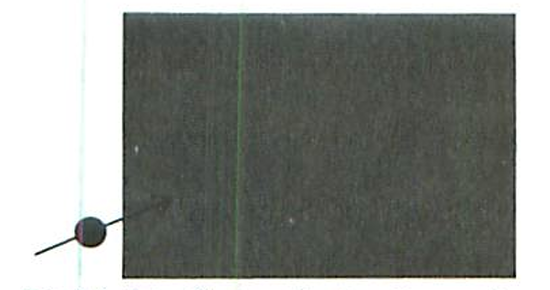
\includegraphics[width=.8\linewidth]{shot.png}
  \caption{The electron is shot into the gas}
  \label{fig:shot}
\end{subfigure}
\begin{subfigure}{.5\textwidth}
  \centering
  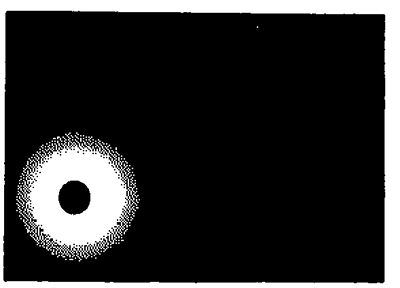
\includegraphics[width=.8\linewidth]{clothing.png}
  \caption{The electron creates holes as it moves along}
  \label{fig:clothing}
\end{subfigure}
\caption{Electron gas propagation taken from \textcite{mattuck_guide_1992}}
\label{fig:propagates}
\end{figure}
As it propagates through this medium, it will have an electrostatic repulsion with the electrons in the gas, so it will create holes (depicted in white) as it moves along (pictured in Figure \ref{fig:clothing}). Therefore, it no longer makes sense to think of the bare electron, but rather the quasi-electron along with its "clothing" of holes. To make this more rigorous, we have the equation
\begin{equation}
    \epsilon_{\text{self}} = \epsilon_{\text{quasi}} - \epsilon_{\text{bare}},
\end{equation}
which is saying that the difference between the quasi-electron energy and the bare electron energy can be thought of as the electron's self-energy, or just the energy of its "clothing". So we can think of $\epsilon_{\text{bare}}$ and $\epsilon_{\text{quasi}}$ as originating from the inverses of the noninteracting and interacting Green's functions $G_0$ and $G$, respectively. The self-energy $\Sigma$ then captures the difference between these two quantities. 
% Typically, $\Sigma$ is designed to capture all of the quantum mechanical effects of the many-body system, including the exchange and correlation effects, so it is often denoted as $\Sigma_{xc}$. One might argue that DFT also contains a $V_{xc}$, but this is often an approximation that doesn't work universally for systems, whereas the $\Sigma_{xc}$ can be systematically improved by considering increasing orders of perturbation theory.
\section{The $GW$ approximation}
In order to solve the Dyson equation in equation \ref{eq:dyson}, we need to make approximations of the self-energy $\Sigma$. By introducing the screened Coulomb potential $W$, which represents the effective electrostatic interaction between electrons (as described above through the concept of the quasi-electron), the polarization function $\tilde{\chi}$, which describes the response of the system to the introduction of an electron, and the vertex function $\Gamma$, which describes the interaction between the electrons and holes, we get the five Hedin's equations\autocite{hedin_new_1965}, which interrelate these quantities and is presented by the schematic in figure \ref{fig:hedin}, for the sake of brevity. The $GW$ approximation is a simplification of these equations, where we neglect the vertex function $\Gamma$ by setting $\Gamma(1,2,3) = \delta(1,2) \delta(1,3)$.
\begin{figure}
    \centering
    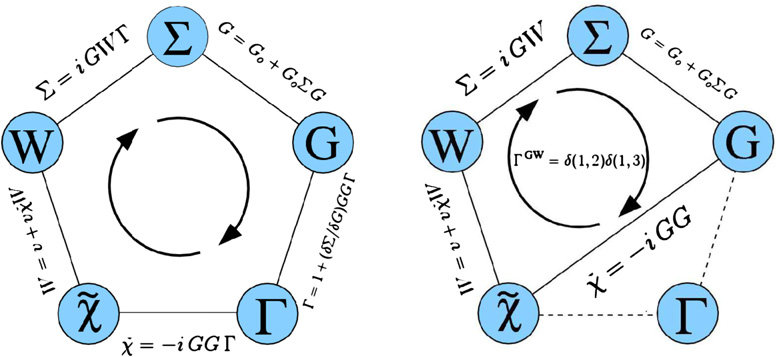
\includegraphics[width=\textwidth]{Left-panel-Graphical-representation-of-Hedins-equations-Right-panel-The-four-coupled.jpg}
    \caption{Graphical representation of Hedin's equations taken from \textcite{noauthor_frontiers_nodate}. The left panel shows the full set of equations, whereas the right panel shows the $GW$ approximation.}
    \label{fig:hedin}
\end{figure}
Full self-consistency, including the vertex function $\Gamma$, is shown in the left panel, whereas the $GW$ approximation, which makes the simple approximation for the vertex function, and therefore neglects it, is shown in the right panel. 
%A cheap person of the $GW$ approximation is the one shot $G_0W_0$ procedure, in which only a single lope of the cycle in figure \ref{fig:hedin} is performed. However, it has been shown that this yields a strong starting pond dependence on the initial KS-DFT calculation. Recently, the linearized $G_0W_0$ density matrix has been proposed by Bruneval and Marques, which has been shown to yield toto energies comparable with fully self consistent flavors of the $GW$ approximation. For example, Geneva proposes a Galitskii-Migdal total energy functional, which uses the linearized $G_0W_0$ density matrix, the noted $\gamma ^{GW}$. Furthermore, he has also extended the the noised $G_0W_0$ density matrix to 
\section{The Bethe-Salpeter equation}
The Bethe-Salpeter equation (BSE) does not neglect the vertex function as in the $GW$ approximation. The upshot of this is that instead of dealing with a single-particle Green's function, as defined in equation \ref{eq:greens}, we now deal with a two-particle Green's function
\begin{equation}
  G_2\left(1,2 ; 1^{\prime}, 2^{\prime}\right)=-i\left\langle\Psi_0\left|T\left[\psi\left(1\right) \psi\left(2\right) \psi^{\dagger}\left(1^{\prime}\right) \psi^{\dagger}\left(2^{\prime}\right)\right]\right| \Psi_0\right\rangle,
\end{equation}
where we define combined spacetime coordinates $1=(\mathbf{r}_1, t_1)$, and so on. This now defines a probability of two particles being created and destroyed at different spacetime coordinates. The electron-hole correlation function\autocite{reining_10_nodate} that one gets from solving the BSE is given by
\begin{equation}
L\left(1,2 ; 1^{\prime}, 2^{\prime}\right)=-G_2\left(1,2 ; 1^{\prime}, 2^{\prime}\right)+G\left(1,1^{\prime}\right) G\left(2,2^{\prime}\right).
\end{equation}
It does not merely describe excitations and the excitations, as we showed the RPA can only do given that it is a single-particle process, but now because we are measuring a two-particle process, we can determine the probability of creating an electron and hole, and also describe the interaction between them. This is imperative for describing excitons.
\section{Outlook}
The $G_0W_0$ procedure constitutes only a single shot of the $GW$ approximation; it only does a single cycle of the right panel in figure \ref{fig:hedin}. Due to its one-shot nature, it shows a strong starting point dependence on the noninteracting Green's function $G_0$, but it is computationally cheap due to not participating in the full self-consistent cycle of figure \ref{fig:hedin}. The linearized $G_0W_0$ density matrix has been proposed by \textcite{bruneval_assessment_2019}, which has been shown to yield total energies comparable with fully self-consistent flavors of the $GW$ approximation\autocite{bruneval_improved_2021} and it has also been implemented to predict properties of solids with success\autocite{denawi_gw_2023}. Perhaps, this could be extended to the BSE and thus provide an accurate description of excitonic correlations at the reduced scaling of a one-shot computation. The concept of matrix product states has recently been applied to the quantum many-body problem\autocite{schollwock_density-matrix_2011}, so it would be interesting to see if one could exploit some locality of the BSE, in order to apply the MPS.
\printbibliography[heading=bibintoc]
\end{document}